\documentclass[12pt]{article}

\usepackage[T1]{fontenc}
\usepackage[utf8]{inputenc}
\usepackage[american]{babel}
\usepackage{lmodern}
\usepackage{geometry}
\geometry{margin=1in}
\usepackage{setspace}
\doublespacing
\usepackage{microtype}
\emergencystretch=2em
\usepackage[section]{placeins}
\usepackage[switch,modulo]{lineno}
\setlength\linenumbersep{10pt}
\renewcommand\linenumberfont{\normalfont\small\ttfamily}

\usepackage{amsmath,amssymb}
\usepackage{graphicx}
\usepackage{booktabs}
\usepackage{threeparttable}
\usepackage{array}
\usepackage{tabularx}
\usepackage{caption}
\usepackage{float}
\usepackage{ragged2e}
\usepackage{siunitx}
\usepackage{xcolor}
\usepackage{tikz}
\usetikzlibrary{arrows.meta,positioning,shapes.geometric}

\sisetup{
  detect-weight,
  detect-family,
  table-number-alignment=center,
  group-separator={\,},
  group-minimum-digits=4
}
\captionsetup{font=small,justification=raggedright,singlelinecheck=false}
\newcolumntype{Y}{>{\RaggedRight\arraybackslash}X}
\newcolumntype{Z}{>{\centering\arraybackslash}X}
\newcolumntype{P}[1]{>{\RaggedRight\arraybackslash}p{#1}}
\renewcommand{\arraystretch}{1.15}
% Keep every manuscript table at one readable font size and one text-width
% footprint; scaling each table to the page independently makes sparse tables
% appear much larger than wide tables.
\newcommand{\tableformat}{\scriptsize\setlength{\tabcolsep}{1pt}}

\usepackage{authblk}
\usepackage{csquotes}
\usepackage[style=apa,backend=biber,maxcitenames=2,uniquelist=false]{biblatex}
\DeclareLanguageMapping{american}{american-apa}
\addbibresource{references.bib}
\usepackage{xurl}
\usepackage[unicode,breaklinks=true]{hyperref}
\hypersetup{colorlinks=true,urlcolor=blue,linkcolor=black,citecolor=black}

% The analysis writes authoritative manuscript artifacts to its build output.
\newcommand{\GeneratedRoot}{results/revision-v1}
\IfFileExists{\GeneratedRoot/results_macros.tex}{%
  % Generated by citation_analysis.py; do not edit manually.
\newcommand{\AnalysisVersion}{revision-v1}
\newcommand{\MatchedPairCount}{102,626}
\newcommand{\ExactHFivePairCount}{64,176}
\newcommand{\MaximumAbsoluteHFiveDifference}{2}
\newcommand{\HFiveCaliperViolationCount}{0}
\newcommand{\PrimaryCoauthorCitationRatePairCount}{74,690}
\newcommand{\PrimaryCoauthorCitationRateCaseMedian}{0.000}
\newcommand{\PrimaryCoauthorCitationRateControlMedian}{0.028}
\newcommand{\PrimaryCoauthorCitationRateMedianDifference}{0.000}
\newcommand{\PrimaryCoauthorCitationRateMeanDifference}{0.048}
\newcommand{\PrimaryCoauthorCitationRateBootstrapCILow}{0.000}
\newcommand{\PrimaryCoauthorCitationRateBootstrapCIHigh}{0.000}
\newcommand{\PrimaryCoauthorCitationRateMeanBootstrapCILow}{0.047}
\newcommand{\PrimaryCoauthorCitationRateMeanBootstrapCIHigh}{0.050}
\newcommand{\PrimaryCoauthorCitationRateRankBiserial}{0.140}
\newcommand{\PrimaryCoauthorCitationRateBHAdjustedP}{0.0000}
\newcommand{\PrimaryCoauthorCitationRateSignFlipP}{0.0001}
\newcommand{\PrimaryReciprocityPairCount}{39,441}
\newcommand{\PrimaryReciprocityCaseMedian}{0.000}
\newcommand{\PrimaryReciprocityControlMedian}{0.000}
\newcommand{\PrimaryReciprocityMedianDifference}{0.000}
\newcommand{\PrimaryReciprocityMeanDifference}{0.096}
\newcommand{\PrimaryReciprocityBootstrapCILow}{0.000}
\newcommand{\PrimaryReciprocityBootstrapCIHigh}{0.000}
\newcommand{\PrimaryReciprocityMeanBootstrapCILow}{0.092}
\newcommand{\PrimaryReciprocityMeanBootstrapCIHigh}{0.100}
\newcommand{\PrimaryReciprocityRankBiserial}{0.341}
\newcommand{\PrimaryReciprocityBHAdjustedP}{0.0000}
\newcommand{\PrimaryReciprocitySignFlipP}{0.0001}
\newcommand{\PrimaryLocalClusteringPairCount}{102,626}
\newcommand{\PrimaryLocalClusteringCaseMedian}{0.000}
\newcommand{\PrimaryLocalClusteringControlMedian}{0.000}
\newcommand{\PrimaryLocalClusteringMedianDifference}{0.000}
\newcommand{\PrimaryLocalClusteringMeanDifference}{0.081}
\newcommand{\PrimaryLocalClusteringBootstrapCILow}{0.000}
\newcommand{\PrimaryLocalClusteringBootstrapCIHigh}{0.000}
\newcommand{\PrimaryLocalClusteringMeanBootstrapCILow}{0.079}
\newcommand{\PrimaryLocalClusteringMeanBootstrapCIHigh}{0.084}
\newcommand{\PrimaryLocalClusteringRankBiserial}{0.264}
\newcommand{\PrimaryLocalClusteringBHAdjustedP}{0.0000}
\newcommand{\PrimaryLocalClusteringSignFlipP}{0.0001}
\newcommand{\PrimaryOutgoingHhiPairCount}{74,690}
\newcommand{\PrimaryOutgoingHhiCaseMedian}{0.074}
\newcommand{\PrimaryOutgoingHhiControlMedian}{0.030}
\newcommand{\PrimaryOutgoingHhiMedianDifference}{0.036}
\newcommand{\PrimaryOutgoingHhiMeanDifference}{0.097}
\newcommand{\PrimaryOutgoingHhiBootstrapCILow}{0.035}
\newcommand{\PrimaryOutgoingHhiBootstrapCIHigh}{0.037}
\newcommand{\PrimaryOutgoingHhiMeanBootstrapCILow}{0.095}
\newcommand{\PrimaryOutgoingHhiMeanBootstrapCIHigh}{0.099}
\newcommand{\PrimaryOutgoingHhiRankBiserial}{0.594}
\newcommand{\PrimaryOutgoingHhiBHAdjustedP}{0.0000}
\newcommand{\PrimaryOutgoingHhiSignFlipP}{0.0001}
\newcommand{\SecondarySelfCitationRatePairCount}{75,526}
\newcommand{\SecondarySelfCitationRateCaseMedian}{0.000}
\newcommand{\SecondarySelfCitationRateControlMedian}{0.007}
\newcommand{\SecondarySelfCitationRateMedianDifference}{0.000}
\newcommand{\SecondarySelfCitationRateMeanDifference}{0.033}
\newcommand{\SecondarySelfCitationRateBootstrapCILow}{0.000}
\newcommand{\SecondarySelfCitationRateBootstrapCIHigh}{0.000}
\newcommand{\SecondarySelfCitationRateMeanBootstrapCILow}{0.031}
\newcommand{\SecondarySelfCitationRateMeanBootstrapCIHigh}{0.034}
\newcommand{\SecondarySelfCitationRateRankBiserial}{0.177}
\newcommand{\SecondarySelfCitationRateBHAdjustedP}{0.0000}
\newcommand{\SecondarySelfCitationRateSignFlipP}{0.0001}
\newcommand{\SecondaryJournalEndogamyPairCount}{79,700}
\newcommand{\SecondaryJournalEndogamyCaseMedian}{0.008}
\newcommand{\SecondaryJournalEndogamyControlMedian}{0.064}
\newcommand{\SecondaryJournalEndogamyMedianDifference}{-0.027}
\newcommand{\SecondaryJournalEndogamyMeanDifference}{-0.009}
\newcommand{\SecondaryJournalEndogamyBootstrapCILow}{-0.027}
\newcommand{\SecondaryJournalEndogamyBootstrapCIHigh}{-0.026}
\newcommand{\SecondaryJournalEndogamyMeanBootstrapCILow}{-0.010}
\newcommand{\SecondaryJournalEndogamyMeanBootstrapCIHigh}{-0.007}
\newcommand{\SecondaryJournalEndogamyRankBiserial}{-0.235}
\newcommand{\SecondaryJournalEndogamyBHAdjustedP}{0.0000}
\newcommand{\SecondaryJournalEndogamySignFlipP}{0.0001}
\newcommand{\SecondaryWithinSampleCitationBalancePairCount}{59,924}
\newcommand{\SecondaryWithinSampleCitationBalanceCaseMedian}{0.000}
\newcommand{\SecondaryWithinSampleCitationBalanceControlMedian}{-0.024}
\newcommand{\SecondaryWithinSampleCitationBalanceMedianDifference}{0.000}
\newcommand{\SecondaryWithinSampleCitationBalanceMeanDifference}{-0.020}
\newcommand{\SecondaryWithinSampleCitationBalanceBootstrapCILow}{0.000}
\newcommand{\SecondaryWithinSampleCitationBalanceBootstrapCIHigh}{0.000}
\newcommand{\SecondaryWithinSampleCitationBalanceMeanBootstrapCILow}{-0.028}
\newcommand{\SecondaryWithinSampleCitationBalanceMeanBootstrapCIHigh}{-0.011}
\newcommand{\SecondaryWithinSampleCitationBalanceRankBiserial}{-0.018}
\newcommand{\SecondaryWithinSampleCitationBalanceBHAdjustedP}{0.0003}
\newcommand{\SecondaryWithinSampleCitationBalanceSignFlipP}{0.0001}
\newcommand{\SecondaryAnnualDyadicSurgeSharePairCount}{75,526}
\newcommand{\SecondaryAnnualDyadicSurgeShareCaseMedian}{0.123}
\newcommand{\SecondaryAnnualDyadicSurgeShareControlMedian}{0.069}
\newcommand{\SecondaryAnnualDyadicSurgeShareMedianDifference}{0.047}
\newcommand{\SecondaryAnnualDyadicSurgeShareMeanDifference}{0.094}
\newcommand{\SecondaryAnnualDyadicSurgeShareBootstrapCILow}{0.046}
\newcommand{\SecondaryAnnualDyadicSurgeShareBootstrapCIHigh}{0.048}
\newcommand{\SecondaryAnnualDyadicSurgeShareMeanBootstrapCILow}{0.092}
\newcommand{\SecondaryAnnualDyadicSurgeShareMeanBootstrapCIHigh}{0.096}
\newcommand{\SecondaryAnnualDyadicSurgeShareRankBiserial}{0.526}
\newcommand{\SecondaryAnnualDyadicSurgeShareBHAdjustedP}{0.0000}
\newcommand{\SecondaryAnnualDyadicSurgeShareSignFlipP}{0.0001}
\newcommand{\PrimarySignificantCount}{4}
\newcommand{\PrimaryMinimumPairCount}{39,441}
\newcommand{\PrimaryMaximumPairCount}{102,626}
\newcommand{\PrimaryFindingText}{All four primary mean differences favored Cases; all four comparisons were significant after adjustment, and 3 median differences were zero.}
\newcommand{\PrimaryDetailedFindingText}{The four primary mean paired differences were Coauthor-citation rate 0.048, 95\% bootstrap CI [0.047, 0.050]; Reciprocity 0.096, 95\% bootstrap CI [0.092, 0.100]; Local clustering 0.081, 95\% bootstrap CI [0.079, 0.084]; Outgoing HHI 0.097, 95\% bootstrap CI [0.095, 0.099]. 3 median differences were zero. Outgoing HHI had a median paired difference of 0.036, 95\% bootstrap CI [0.035, 0.037].}
\newcommand{\SecondaryDetailedFindingText}{The median difference in same-journal referencing was -0.027, 95\% CI [-0.027, -0.026]; the median difference in the maximum year-to-year increase to one recipient was 0.047, 95\% CI [0.046, 0.048].}
\newcommand{\SensitivityFindingText}{The exact-$h_5$ check had positive mean differences for all four primary comparisons; outgoing HHI had a median difference of 0.034 (95\% CI [0.033, 0.035]). Using the same-year coauthor definition, the median difference was 0.000 (95\% CI [0.000, 0.000]).}
\newcommand{\EligibleCaseCount}{75,954}
\newcommand{\EligibleControlCount}{99,889}
\newcommand{\ScreenableCaseCount}{53,365}
\newcommand{\ScreenableControlCount}{71,146}
\newcommand{\FlaggedCaseCount}{1,880}
\newcommand{\FlaggedControlCount}{162}
\newcommand{\TotalFlaggedCount}{2,042}
\newcommand{\CaseShareAmongFlagsPercent}{92.07}
\newcommand{\FlaggedCasePercent}{2.48}
\newcommand{\FlaggedControlPercent}{0.16}
\newcommand{\CaseControlEnrichment}{15.26}
\newcommand{\AnomalyFisherP}{0.0000}
\newcommand{\AnomalyScreenableCount}{124,511}
\newcommand{\DetectorThresholdCount}{5,972}
\newcommand{\DetectorThresholdPercent}{4.80}
\newcommand{\CohesionConfirmationCount}{2,056}
\newcommand{\CohesionConfirmationPercent}{1.65}
\newcommand{\DetectorConfirmationOverlapCount}{2,042}
\newcommand{\DetectorConfirmationOverlapPercent}{1.64}
\newcommand{\DetectorOnlyCount}{3,930}
\newcommand{\CohesionOnlyCount}{14}
\newcommand{\DetectorCohesionSpearmanN}{124,511}
\newcommand{\DetectorCohesionSpearmanRho}{0.421}
\newcommand{\DetectorCohesionSpearmanP}{0.0000}
\newcommand{\AnomalyFeatureAblationFlaggedMinimum}{1901}
\newcommand{\AnomalyFeatureAblationFlaggedMaximum}{2056}
\newcommand{\AnomalyFeatureAblationJaccardMinimum}{0.931}
\newcommand{\AnomalyFeatureAblationJaccardMaximum}{0.995}
\newcommand{\AnomalyFeatureAblationEnrichmentMinimum}{14.83}
\newcommand{\AnomalyFeatureAblationEnrichmentMaximum}{15.58}
\newcommand{\AnomalyOverlapFindingText}{The two screen rules agreed for 2,042 rows; 3,930 passed only the first rule and 14 only the second. Their scores were positively related ($\rho=0.421$, $p<0.001$).}
\newcommand{\AnomalyFeatureAblationFindingText}{Removing one input at a time changed little: flag overlap ranged from 0.931 to 0.995, and Case/Control enrichment ranged from 14.83 to 15.58.}
\newcommand{\AnomalyFindingText}{The screen flagged 2.48\% of Case rows and 0.16\% of Control rows, a 15.26-fold difference.}
\newcommand{\AnomalyDetailedFindingText}{The screen flagged 1880 Cases and 162 Controls (2.48\% versus 0.16\%; 15.26-fold difference; Fisher exact $p<0.001$).}
\newcommand{\WithinTierMixingPercent}{94.03}
\newcommand{\TierMixingAssortativity}{0.828}
\newcommand{\TierMixingPermutationP}{0.0001}
\newcommand{\MixingFindingText}{94.03\% of matched citation weight stayed within the same group (label-swap $p<0.001$).}
\newcommand{\OutlierComponentCount}{5}
\newcommand{\LargestOutlierComponentSize}{6}
\newcommand{\ComponentFindingText}{5 outlier components contained at least five nodes; the largest contained 6 nodes.}
\newcommand{\CliqueStructuralCount}{36311}
\newcommand{\CliqueReciprocalCount}{9362}
\newcommand{\CliqueUniqueMemberCount}{15177}
\newcommand{\CliqueCaseMemberCount}{11252}
\newcommand{\CliqueControlMemberCount}{3925}
\newcommand{\CliqueCaseMembershipPercent}{10.96}
\newcommand{\CliqueControlMembershipPercent}{3.82}
\newcommand{\CliquePairedDifferencePoints}{7.14}
\newcommand{\CliqueCaseOnlyPairs}{10678}
\newcommand{\CliqueControlOnlyPairs}{3351}
\newcommand{\CliqueDiscordantPairs}{14029}
\newcommand{\CliqueExactP}{<0.001}
\newcommand{\CliqueSubjectsCaseHigher}{5}
\newcommand{\CliqueSubjectsControlHigher}{0}
\newcommand{\CliqueSubjectsTied}{0}
\newcommand{\CliqueFindingText}{Primary-rule reciprocal-clique membership was 10.96\% for Cases and 3.82\% for Controls (paired difference 7.14 percentage points; exact $p<0.001$).}
%
}{ }

% These defaults make a draft compile before the full database rebuild.  They
% contain no numerical result and are replaced by generated macros when the
% canonical analysis has completed.
\providecommand{\MatchedPairCount}{\num{9431}}
\providecommand{\MaximumAbsoluteHFiveDifference}{pending}
\providecommand{\HFiveCaliperViolationCount}{pending}
\providecommand{\PrimaryFindingText}{Primary estimates are pending the canonical full-data rebuild.}
\providecommand{\PrimaryDetailedFindingText}{Primary estimates are pending the canonical full-data rebuild.}
\providecommand{\SecondaryDetailedFindingText}{Secondary estimates are pending the canonical full-data rebuild.}
\providecommand{\SensitivityFindingText}{Sensitivity estimates are pending the canonical full-data rebuild.}
\providecommand{\AnomalyFindingText}{Anomaly-enrichment estimates are pending the canonical full-data rebuild.}
\providecommand{\AnomalyDetailedFindingText}{Anomaly-enrichment estimates are pending the canonical full-data rebuild.}
\providecommand{\AnomalyOverlapFindingText}{Detector--restriction overlap estimates are pending the canonical full-data rebuild.}
\providecommand{\AnomalyFeatureAblationFindingText}{Feature-ablation estimates are pending the canonical full-data rebuild.}
\providecommand{\MixingFindingText}{Tier-mixing estimates are pending the canonical full-data rebuild.}
\providecommand{\CliqueFindingText}{Formal clique results are reported in the generated tables.}
\providecommand{\CliqueNullMeanCaseSharePercent}{pending}

\newcommand{\artifactpending}[1]{%
  \fbox{\begin{minipage}{0.88\linewidth}\centering
  \textit{Generated artifact pending.  No earlier estimate is substituted.}
  \end{minipage}}%
}
\newcommand{\inputgeneratedtable}[3]{%
  \IfFileExists{\GeneratedRoot/tables/#1.tex}{%
    \input{\GeneratedRoot/tables/#1.tex}%
  }{%
    \begin{table}[H]
      \centering
      \caption{#3}
      \label{#2}
      \artifactpending{tables/#1.tex}
    \end{table}%
  }%
}

\title{Citation-Network Cohesion and Reciprocal Citation Cliques Across Journal-Impact Groups:\\
A Matched Author Analysis}
\author{Panagiotis-Alexios Spanakis}
\author{Grigorios Alexandrou}
\author{Diomidis Spinellis}
\affil{Department of Management Science and Technology,
Athens University of Economics and Business (AUEB), Athens, Greece}
\date{}

\begin{document}
\maketitle
\linenumbers

\begin{abstract}
We ask whether authors in lower-impact journal groups have different citation patterns from matched authors in higher-impact groups.  We call the lower-impact observations Cases and the higher-impact observations Controls.  We compare \MatchedPairCount\ author--subject pairs within subject and at similar recent citation productivity.  Cases had higher average values on all four primary measures, although three median differences were zero because many pairs tied at zero.  A defined clique analysis, in which every member pair is linked and many links are returned, found \CliqueReciprocalCount\ reciprocal cliques among \CliqueStructuralCount\ candidate groups; randomized graphs averaged \CliqueNullMeanCount\ reciprocal cliques (empirical $p=\CliqueNullP$), and \CliqueCaseSharePercent\% of clique memberships were Cases (label-swap $p=\CliqueLabelSwapP$).  The results support a directional structural association between journal-impact group and citation-network organization.
\end{abstract}

\noindent\textbf{Keywords:} scientometrics; citation networks; matched design; network cohesion; journal impact; anomaly screening

\section{Introduction}
\label{sec:introduction}

Citation indicators are widely used to summarize scholarly influence, allocate resources, and support evaluation.  Their convenience also creates incentives to optimize what is measured, which can weaken the connection between an indicator and the quality it is intended to represent \parencite{Goo84,Hicks2015,Biagioli2019}.  Excessive self-citation, coercive citation, and concentrated citation exchange are therefore important objects of measurement in their own right \parencite{Wilhite2012,VanNoorden2019,Biagioli2020}.

Most evidence on unusual citation structure is either journal-level or begins with groups already selected for unusual behavior.  Journal-network studies can identify exceptional exchange patterns \parencite{Kojaku2021}, and analyses of citation stacking show how journal-level citation flows can be distorted \parencite{heneberg2016}.  Author-level concentration indicators can show when a small set of collaborators accounts for much of an author's citation impact \parencite{Evdaimon2024}.  Less is known about whether simple author-network measures differ across journal-impact groups after authors are compared within subject and at similar levels of recent citation productivity.

This study addresses that gap with a matched author--subject design.  Low-impact and high-impact refer only to groups defined by subject-specific, publication-weighted 25th and 75th percentile cutoffs of journal Eigenfactor scores.  We use \emph{Case} and \emph{Control} as compact labels for those operational groups; neither label evaluates the scientific merit of an author or work.

The study asks three questions:
\begin{enumerate}
  \item Do matched Case and Control authors differ in citation-network cohesion and outgoing citation concentration?
  \item Are author--subject profiles that are unusual relative to Controls enriched among Cases?
  \item How do fractional citation weights mix across the two groups?
\end{enumerate}

We expect Case author--subjects to have higher values than Controls on four primary measures: citations to previous collaborators, reciprocal citation, local neighbor connections, and concentration of outgoing citations.  This is an associational hypothesis, not a causal or integrity claim.  Because many values are zero, a zero median shift does not rule out a directional difference.  Network closure can reflect legitimate specialization and collaboration, so the anomaly procedure is a screening device.

\section{Related Work}
\label{sec:related-work}

Research evaluation based on citation counts, the $h$-index, and journal indicators has long been accompanied by cautions about field differences and strategic responses \parencite{Gar06,Hirsch2005,Hicks2015}.  Self-citation is common and can be substantively appropriate, but extreme rates complicate comparisons \parencite{Aksnes2003,VanNoorden2019}.  Coercive citation and metric gaming demonstrate that observed references can also respond to editorial and institutional incentives \parencite{Wilhite2012,Baccini2019}.

Several strands of work motivate a network perspective.  Kojaku et al.\ identify anomalous groups in journal citation networks by comparing observed patterns with network expectations \parencite{Kojaku2021}.  Heneberg examines the transition from journal self-citation to citation stacking through journal-level citation flows \parencite{heneberg2016}.  These approaches establish the value of relational structure but operate at the venue level.  At the author level, Evdaimon et al.\ propose indicators based on the concentration of citing authors and hyper-collaboration \parencite{Evdaimon2024}.  Their concentration measures identify a narrow citing base; local closure, reciprocity, and concentration of an author's own references provide complementary information about how that base is connected.

The present analysis combines this network perspective with within-subject author matching.  It does not attempt to classify behavior as legitimate or illegitimate.  Instead, it estimates matched differences in a small, declared set of network measures and applies a Control-referenced screen whose output remains explicitly descriptive.

\section{Data and Cohort}
\label{sec:data-cohort}

\subsection{Source data and study window}

The source is a fixed Crossref snapshot processed with \textit{alexandria3k} \parencite{Spinellis2023}.  The study window covers citing and cited works dated 2020--2024.  Available fields include Digital Object Identifiers (DOIs), publication year, normalized journal International Standard Serial Numbers (ISSNs), work references, and author rows with optional ORCID researcher identifiers.  ORCID is a persistent identifier for a researcher.  The estimates apply to this fixed snapshot and to the author--subject observations that meet the stated inclusion criteria.

Journals are assigned to Health Sciences, Life Sciences, Physical Sciences, Social Sciences and Humanities, or Multidisciplinary.  The existing classification uses a deterministic, cached large-language-model annotation of representative journal content.

The retained venue classification uses fixed subject-specific journal scores from a separate directed journal-citation calculation \parencite{West2008}.  An Eigenfactor score is a journal influence score based on citation flows.  In plain terms, the calculation passes influence from citing journals to cited journals, excludes journal self-citations, and uses article counts to redistribute influence from journals without outgoing citations and to restart the calculation.  These journal-level scores define the two venue groups; they are an input to the comparison, not an author-network outcome.  The exact matrix specification is given in Appendix~\ref{app:venue-scores}.

The current workflow consumes the fixed database scores as an upstream exposure rather than re-estimating them.  After scores are attached to eligible 2020--2024 work rows, the 25th and 75th percentile cutoffs are calculated across positive-score work rows within each subject.  A journal therefore contributes once per eligible work: the cutoffs are publication weighted, not percentiles over distinct journals.  Journals at or below the lower cutoff form the low-impact group and those at or above the upper cutoff form the high-impact group.  No new venue classification was undertaken for this revision.

\subsection{Author--subject cohort}

The unit used throughout is an \emph{author--subject}, meaning one researcher considered within one subject area, identified by $(\mathrm{ORCID},s)$.  An author is a Case in subject $s$ when at least 70\% of eligible works in that subject appear in low-impact journals, and a Control when at least 70\% appear in high-impact journals.  Authors not meeting either rule are excluded from matching.  A uniqueness check prevents more than one group assignment for the same $(\mathrm{ORCID},s)$ key.

The retained primary cohort contains \MatchedPairCount\ matched Case--Control pairs across the five subjects.  The deterministic 10\% ORCID sample and the original matching cohort are retained to separate analytical corrections from cohort redefinition.

\section{Matching}
\label{sec:matching}

Recent subject-specific citation productivity is summarized by $h_5$, the Hirsch index calculated from an author's works in subject $s$ published during 2020--2024 \parencite{Hirsch2005}.  In ordinary language, $h_5$ is the largest number of works that each have at least that many citations in the fixed snapshot.  The retained upstream table contains only positive values, so this fixed-cohort revision restricts the matching pool to $h_5\geq1$ and excludes otherwise group-eligible zero-$h_5$ profiles before candidate generation.

We pair lower-impact and higher-impact author--subjects within the same subject when their $h_5$ values differ by at most three points.  Candidates are considered in the fixed order subject, smallest absolute $h_5$ difference, Case ORCID, and Control ORCID; each author--subject can be used only once.

An independent audit rebuilds this process from the source profiles and compares it with the retained cohort.  It reproduced the retained pair membership exactly within the positive-$h_5$ pool; no pair exceeded the three-point limit and no author--subject key was reused.  The complete audit accompanies the replication materials.

The matching table supplies the Case ORCID, Control ORCID, subject, and both $h_5$ values.  Feature rows are linked back to this table twice, on $(\mathrm{case\_orcid},s)$ and $(\mathrm{control\_orcid},s)$; ORCID-only joins are not used.

We report the distribution of $h_5$ and the within-pair difference before outcome testing.  Because residual differences can remain under caliper matching, the four primary comparisons are repeated on the subset with exact $h_5$ equality.

\inputgeneratedtable{matching_balance}{tab:matching-balance}{Matched authors and balance by subject.}

The generated cohort audit found a maximum observed absolute $h_5$ difference of \MaximumAbsoluteHFiveDifference\ and \HFiveCaliperViolationCount\ pairs beyond the three-point caliper.

\section{Network Construction and Definitions}
\label{sec:network-construction}

We represent authors as nodes and citations as links between nodes.  A link has a direction, from the citing author to the cited author, and a fractional weight that accounts for the number of authors on both works.  We use the word ``network'' for this set of nodes and weighted links.

\subsection{Reference resolution and fractional weights}

A citing-work/cited-work DOI pair is deduplicated before either work is expanded to author rows.  Let $n_c$ and $n_a$ be the complete counts of author rows on the citing and cited work.  These denominators include authors without ORCIDs.  A resolved work citation contributes
\begin{equation}
  \frac{1}{n_c n_a}
\end{equation}
to each identified citing-author/identified cited-author combination.  Rows with an unidentified endpoint do not produce analytic author edges; in particular, missing identifiers cannot become a shared pseudo-author.  Multiple matched authors on one citing work do not multiply the underlying resolved work reference.

Every analytic edge is keyed by subject, citing ORCID, cited ORCID, and citation year.  Only citing works assigned to the matched author's subject contribute to that author--subject's measures.  Duplicate rows are aggregated so that this key is unique.

For coauthor classification, let $c_{ij}$ be the first year in which authors $i$ and $j$ published together.  A citation from $i$ to $j$ in year $t$ is a prior-coauthor citation only if $c_{ij}<t$.  A sensitivity analysis uses $c_{ij}\leq t$ to show the effect of admitting same-year collaborations.

\subsection{Graph and reference populations}

The analysis uses three views of the citation links so that each measure has a clear population.
\begin{description}
  \item[Each author's outgoing links.] For each matched author--subject $i$, this view contains citations from $i$ to any identified author reached from an eligible citing work.  It defines self-citation, citations to previous collaborators, outgoing concentration, and the largest year-to-year increase to one recipient.
  \item[Links among matched authors.] For each subject $s$, this view retains only matched authors and the links between them.  It defines reciprocal citation, local neighbor connections, the balance of incoming and outgoing weight, and citation mixing between the two groups.
  \item[Deduplicated work references.] This view is built before author expansion and defines same-journal referencing even when the cited author is not identified.
\end{description}
Keeping these views separate prevents a measure based on all identified recipients or work references from being mistaken for a measure based only on matched authors.

\subsection{Notation, metrics, and missing values}

Some measures follow an author's outgoing citations to any identified recipient; others use only links between matched authors.  Direction is ignored only for the simple neighbor graph used for local clustering.

Let $x_{ijt}$ denote the fractional citation weight from author $i$ to author $j$ in year $t$, after the construction above.  Missing dyad--years are zero, and $w_{ij}=\sum_{t=2020}^{2024}x_{ijt}$ is cumulative weight.  If $V_s$ is the set of matched authors in subject $s$, the matched-author graph is the directed, weighted, loopless graph
\begin{equation}
  G_s=(V_s,E_s,w),\qquad
  E_s=\{(i,j):i,j\in V_s,\ i\ne j,\ w_{ij}>0\}.
\end{equation}
Its simple binary undirected projection is
\begin{equation}
  U_s=(V_s,\widetilde E_s),\qquad
  \{i,j\}\in\widetilde E_s
  \Longleftrightarrow i\ne j\ \text{and}\ w_{ij}+w_{ji}>0.
\end{equation}
Direction and fractional weight are discarded only in $U_s$.  Self-edges remain available in the outgoing ego layer for self-citation and surge share but do not enter $G_s$ or its peer-network measures.

\subsection{Formal reciprocal-clique analysis}
\label{sec:clique-analysis}

We test citation-clique structure on all matched authors, not only on authors flagged by the screen.  A clique $C$ is a group of at least four matched authors in which every pair is connected by a citation in at least one direction.  We keep only maximal groups, meaning that no additional matched author can be added without breaking that rule.  The direction and weight of the links are then evaluated separately.  For a clique of size $k$, directed density is
\begin{equation}
  d_C=\frac{m_C}{k(k-1)},
\end{equation}
where $m_C$ is the number of positive directed dyads among the $k$ members.  Weighted reciprocity is
\begin{equation}
  r_C=\frac{\sum_{\{i,j\}\subset C}\min(w_{ij},w_{ji})}
           {\sum_{\{i,j\}\subset C}\max(w_{ij},w_{ji})}.
\end{equation}
The primary rule requires at least 75\% of all possible directed links and a weighted reciprocity of at least 0.50.  We repeat it for minimum clique sizes $k=3,4,5$ and reciprocity thresholds $0.25,0.50,0.75$; the density threshold remains fixed at 0.75.  The anomaly flag is reported for these groups but does not define them.

To ask whether the observed count is unusual, we create randomized versions of each subject network.  Each random version keeps every author's number of incoming and outgoing links, but changes which authors are linked.  We then score the same candidate cliques with the same rules.  We use 500 independent random versions and report the proportion that reach or exceed the observed value, with the standard add-one correction.  A separate set of 500 runs swaps Case and Control labels within each matched pair; this tests whether clique membership is concentrated in Cases.  These comparisons test whether the defined pattern is unusual and where it is concentrated.  They do not explain why it occurred.

The study-specific temporal measure is
\begin{equation}
  B_i=
  \frac{\max_{j,t=2021,\ldots,2024}[x_{ijt}-x_{ij,t-1}]_+}
       {\sum_j\sum_{t=2020}^{2024}x_{ijt}}.
  \label{eq:surge-share}
\end{equation}
This study-specific temporal increment is not a state-transition burst-detection model.

\begin{table}[p]
  \centering
  \caption{Declared author--subject measures.}
  \label{tab:metric-definitions}
  \tableformat
  \begin{threeparttable}
  \begin{tabularx}{\textwidth}{@{}P{0.17\textwidth}P{0.36\textwidth}Y@{}}
    \toprule
    Measure & Definition & Population and interpretation \\
    \midrule
    Prior-coauthor citation rate
      & $\displaystyle
        \frac{\sum_{t,j\ne i}x_{ijt}\mathbf{1}(c_{ij}<t)}
        {\sum_{t,j\ne i}x_{ijt}}$
      & Outgoing ego layer.  Fraction of identified non-self outgoing weight directed to an author whose first collaboration preceded the citation year. \\
    \addlinespace
    Self-citation rate
      & $\displaystyle
        \frac{\sum_t x_{iit}}{\sum_{t,j}x_{ijt}}$
      & Outgoing ego layer.  Fraction of identified outgoing weight assigned to the same ORCID. \\
    \addlinespace
    Reciprocity
      & $\displaystyle
        \frac{\sum_{j\ne i}\min(w_{ij},w_{ji})}
        {\sum_{j\ne i}w_{ij}}$
      & Directed, weighted $G_s$.  Among matched peers, the share of outgoing weight that is also returned to the author. \\
    \addlinespace
    Local clustering
      & $\displaystyle \frac{2T_i}{k_i(k_i-1)}$
      & Binary projection $U_s$.  Among an author's matched neighbors, the share of neighbor pairs that are connected to each other. Here $k_i$ is the number of matched neighbors and $T_i$ is the number of connected pairs among those neighbors. \\
    \addlinespace
    Outgoing Herfindahl--\allowbreak Hirschman index (HHI)
      & $\displaystyle \sum_{j\ne i}p_{ij}^{2}$,
        $p_{ij}=w_{ij}/\sum_{k\ne i}w_{ik}$
      & Outgoing ego layer.  Concentration of identified non-self outgoing weight across recipients; values near 1 mean that one recipient receives nearly all of the weight \parencite{Hirschman1964}. \\
    \addlinespace
    Journal endogamy
      & Resolved outgoing work references whose citing and cited journals have the same nonblank normalized ISSN, divided by all resolved outgoing work references
      & Deduplicated work-reference layer.  Share of resolved references whose citing and cited journals have the same normalized ISSN.  This descriptive term does not imply impropriety. \\
    \addlinespace
    Within-sample citation balance
      & $\displaystyle
        \frac{\sum_{j\ne i}w_{ij}-\sum_{j\ne i}w_{ji}}
        {\sum_{j\ne i}w_{ij}+\sum_{j\ne i}w_{ji}}$
      & Directed, weighted $G_s$.  Positive values mean more outgoing than incoming weight among matched peers; negative values mean more incoming weight. \\
    \addlinespace
    Maximum annual dyadic surge share
      & $\displaystyle
        \frac{\max_{\substack{j\\t=2021,\ldots,2024}}[x_{ijt}-x_{ij,t-1}]_+}
        {\sum_j\sum_{t=2020}^{2024}x_{ijt}}$
      & Outgoing ego layer.  Largest year-to-year increase to one recipient, divided by all identified outgoing weight. \\
    \bottomrule
  \end{tabularx}
  \begin{tablenotes}
    \item \textit{Notes.} $x_{ijt}$ is fractional citation weight, $w_{ij}$ is cumulative weight, $c_{ij}$ is the first joint-publication year, and $\mathbf{1}(\cdot)$ is an indicator.  $G_s$ is the directed matched-author graph, $U_s$ is its binary neighbor graph, and $[z]_+=\max(z,0)$.  Measures are calculated separately for each author--subject; the zero and missing-value rules follow the table.
  \end{tablenotes}
  \end{threeparttable}
\end{table}

Unavailable values remain missing through feature assembly.  A zero is used only when the denominator and graph population are observed but the relevant event is absent.  Thus a defined rate with no qualifying citations is zero; reciprocity is zero when internal outgoing weight exists but none is returned; clustering is zero for an observed induced-graph node with fewer than two neighbors; and journal endogamy is zero when resolved references exist but none remains within the citing journal.  Outgoing HHI is missing when there is no identified non-self outgoing weight, balance is missing when total internal incident weight is zero, journal endogamy is missing when no resolved outgoing work reference exists, and surge share is missing when total identified outgoing weight is zero.  These rules imply $0\leq B_i\leq1$.  Statistical comparisons use complete-pair deletion separately for each metric rather than a common imputed matrix.

\begin{figure}[p]
  \centering
  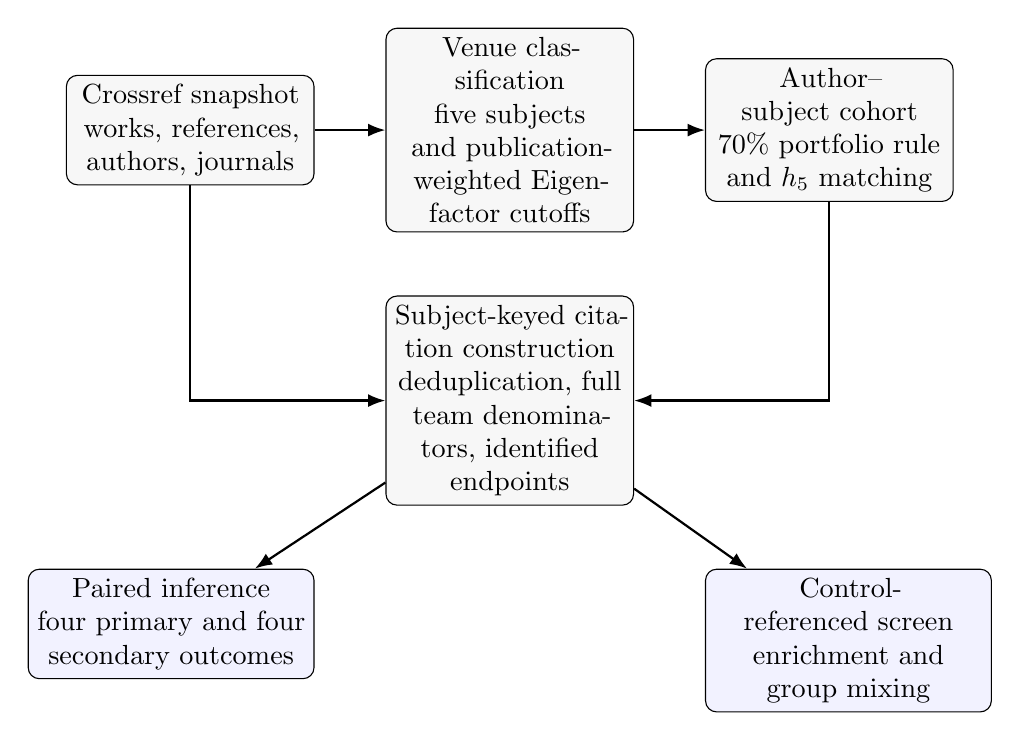
\begin{tikzpicture}[
    node distance=8mm and 9mm,
    box/.style={draw,rounded corners,align=center,text width=0.24\textwidth,minimum height=12mm,fill=black!3},
    branch/.style={draw,rounded corners,align=center,text width=0.28\textwidth,minimum height=13mm,fill=blue!5},
    arrow/.style={-{Latex[length=2.2mm]},thick}
  ]
    \node[box] (data) {Crossref snapshot\\works, references, authors, journals};
    \node[box,right=of data] (venues) {Venue classification\\five subjects and publication-weighted Eigenfactor cutoffs};
    \node[box,right=of venues] (cohort) {Author--subject cohort\\70\% portfolio rule and $h_5$ matching};
    \node[box,below=of venues] (edges) {Subject-keyed citation construction\\deduplication, full team denominators, identified endpoints};
    \node[branch,below left=of edges] (paired) {Paired inference\\four primary and four secondary outcomes};
    \node[branch,below right=of edges] (screen) {Control-referenced screen\\enrichment and group mixing};
    \draw[arrow] (data) -- (venues);
    \draw[arrow] (venues) -- (cohort);
    \draw[arrow] (cohort) |- (edges);
    \draw[arrow] (data) |- (edges);
    \draw[arrow] (edges) -- (paired);
    \draw[arrow] (edges) -- (screen);
  \end{tikzpicture}
  \caption{Reader-facing study design.  Venue classification and author matching define the cohort; subject-keyed citation construction then supports two declared analytical branches.}
  \label{fig:study-design}
\end{figure}

\section{Paired Inference}
\label{sec:paired-inference}

The four primary outcomes are citations to previous collaborators, reciprocal citation, connections among an author's citation neighbors, and outgoing HHI.  HHI is a concentration score from 0 to 1; it is higher when an author sends most outgoing citation weight to a small number of recipients.  The four secondary outcomes are self-citation, same-journal referencing, the balance of incoming and outgoing links, and the largest year-to-year increase to one recipient.  The former normalised burst-intensity feature is not an additional outcome; it was replaced by the surge share in Equation~\ref{eq:surge-share}.  The revised analysis therefore reports eight distinct outcomes in two declared families.

For each matched pair, we subtract the Control value from the Case value.  A positive difference therefore means that the Case value is larger.  Only pairs with both values available enter a comparison.  Because the measures contain many ties and zeros, we use the two-sided paired Wilcoxon signed-rank test, which does not assume a normal distribution \parencite{Wilcoxon1945}.  We report the number of pairs, the median difference, and a rank effect size:
\begin{equation}
  r_{\mathrm{rb}}=\frac{W^+-W^-}{W^++W^-},
\end{equation}
where $W^+$ and $W^-$ add the ranks of positive and negative differences after zero differences are omitted.  The effect ranges from $-1$ to 1; a positive value means that Case ranks tend to be higher.  We obtain 95\% intervals from 2,000 bootstrap samples of matched pairs \parencite{Efron1993}.  We also report mean differences and their bootstrap intervals because they give an intuitive measure of the size of the shift.  Benjamini--Hochberg correction adjusts the four $p$-values in each outcome family for the number of tests \parencite{Benjamini1995}.

As a randomization check, we randomly reverse the sign of each pair difference in 10,000 runs and compare the resulting mean differences with the observed one.  This keeps the size of every pair difference while removing its direction.  We also repeat the primary comparisons for exact-$h_5$ matches and for a definition that counts collaborations formed in the citation year.

\section{Anomaly Screen}
\label{sec:anomaly-screen}

The anomaly analysis asks a different question from the matched comparison: are unusual profiles more common among Cases than among Controls?  It is a screening rule, not a prediction model and not evidence of intent.

An author--subject enters the screen only when it has at least one identified non-self outgoing citation.  The screen uses five measures of an author's citation links: self-reference, citations to previous collaborators, mutual exchange, connections among neighbors, and concentration among recipients.  Same-journal referencing, the balance of incoming and outgoing links, and year-to-year increases are reported separately and are not screen inputs.  All five inputs must be observed; an unavailable value is not changed to zero.  Controls define the subject-specific reference values, and Cases are compared with those values.

An Isolation Forest is a tree-based method that gives a higher score to a profile that is easy to separate from typical Controls \parencite{Liu2008}.  A row passes this part of the screen when its score is above the 99th percentile of Controls in the same subject.  A row also passes the second part when at least two of four cohesion measures exceed their Control percentiles.  The final flag requires both parts.  Because the four cohesion measures also enter the first part, the two parts are related and are not independent evidence.

Sensitivity analyses vary the Control percentile, random seed, and detector feature set.  We report overlap between the detector and cohesion restriction, their rank association, and leave-one-feature-out stability.  These quantities describe an operational screen; they are not measures of classification accuracy because group is not a ground-truth anomaly label.

Finally, we summarize where citation weight goes.  The $2\times2$ table has the citing group in the rows and the cited group in the columns.  Weighted assortativity compares the observed share of same-group citations with the share expected from the row and column totals \parencite{Newman2002}:
\begin{equation}
  r=\frac{\operatorname{tr}(e)-a^\mathsf{T}b}{1-a^\mathsf{T}b}.
\end{equation}
  Here $e$ is the observed $2\times2$ table of citation-weight shares, $a$ contains its row totals, $b$ contains its column totals, and $\operatorname{tr}(e)$ is the observed same-group share.  Positive $r$ indicates more same-group citation weight than expected from those totals.  The reported label-swap $p$-value compares the observed same-group share with 10,000 runs in which the two labels are swapped within each matched pair.  The swaps keep the citation links and matching structure unchanged while removing the original group labels.

\section{Results}
\label{sec:results}

All numerical values in this section come from the same analysis and are shown in the tables and figures.

\subsection{Matched differences in network measures}
\label{sec:paired-results}

The primary and secondary matched comparisons are shown in Tables~\ref{tab:paired-primary} and~\ref{tab:paired-secondary}.

Across the matched pairs, Cases had higher average values on all four primary measures.  Three median differences were zero because many pairs tied at zero; among non-tied pairs, Case values were more often higher.  The result is a shift across the paired sample rather than a larger value for every author.

\inputgeneratedtable{paired_primary}{tab:paired-primary}{Matched comparisons of the four primary measures.}

\inputgeneratedtable{paired_secondary}{tab:paired-secondary}{Matched comparisons of secondary measures.}

\FloatBarrier
\PrimaryDetailedFindingText

\SecondaryDetailedFindingText

\IfFileExists{\GeneratedRoot/figures/paired_effects.pdf}{%
  \begin{figure}[H]
    \centering
    
\includegraphics[width=0.8\linewidth]{\GeneratedRoot/figures/paired_effects.pdf}
    \caption{Matched effect estimates by outcome.  Points show median paired differences and bars show paired-bootstrap 95\% confidence intervals; mean differences and mean intervals are reported in Tables~\ref{tab:paired-primary} and~\ref{tab:paired-secondary}.}
    \label{fig:paired-effects}
  \end{figure}
}{ }

Pair counts are reported separately because the missingness pattern differs by measure.  The count for every metric is checked not to exceed the \MatchedPairCount\ primary pairs.

\subsection{Sensitivity of primary comparisons}

\inputgeneratedtable{exact_h5_sensitivity}{tab:exact-h5}{Checks using exact-$h_5$ matches and same-year collaborations.}

\SensitivityFindingText

The check keeps the direction of the primary results.  The table shows the estimates and intervals for the alternative matching and collaboration definitions.

\subsection{Control-referenced anomaly enrichment}
\label{sec:anomaly-results}

\AnomalyDetailedFindingText

\inputgeneratedtable{anomaly_enrichment}{tab:anomaly-enrichment}{Screen results by journal-impact group.}

\AnomalyOverlapFindingText

\inputgeneratedtable{anomaly_overlap}{tab:anomaly-overlap}{The two screen rules and their overlap.}

\inputgeneratedtable{anomaly_sensitivity}{tab:anomaly-sensitivity}{Sensitivity of screen results.}

\AnomalyFeatureAblationFindingText\ Details appear in Table~\ref{tab:anomaly-feature-ablation}.

\IfFileExists{\GeneratedRoot/figures/anomaly_enrichment.pdf}{%
  \begin{figure}[H]
    \centering
    
\includegraphics[width=0.8\linewidth]{\GeneratedRoot/figures/anomaly_enrichment.pdf}
    \caption{Share of eligible author--subjects flagged in each group under the declared screen.  Values and supporting counts are generated from the same final flag used in all downstream analyses.}
    \label{fig:anomaly-enrichment}
  \end{figure}
}{ }

\subsection{Fractional group mixing}
\label{sec:mixing-results}

\MixingFindingText

\inputgeneratedtable{tier_mixing}{tab:tier-mixing}{Where matched authors cite.}

\IfFileExists{\GeneratedRoot/figures/tier_mixing.pdf}{%
  \begin{figure}[H]
    \centering
    
\includegraphics[width=0.8\linewidth]{\GeneratedRoot/figures/tier_mixing.pdf}
    \caption{Fractional citation-weight mixing between Case and Control nodes.  The comparison distribution is based on within-pair group-label swaps.}
    \label{fig:tier-mixing}
  \end{figure}
}{ }

\subsection{Formal reciprocal-clique structure}
\label{sec:clique-results}

\CliqueFindingText

\inputgeneratedtable{clique_summary}{tab:clique-summary}{Defined reciprocal-clique pattern and randomized comparison.}

\IfFileExists{\GeneratedRoot/figures/clique_nulls.pdf}{%
  \begin{figure}[H]
    \centering
    
\includegraphics[width=0.72\linewidth]{\GeneratedRoot/figures/clique_nulls.pdf}
    \caption{Observed clique results compared with random averages.  The top row shows the number of reciprocal cliques; the bottom row shows the percentage of clique members who are Cases.  Red bars are observed values, gray bars are random averages, and each row reports its empirical $p$-value.}
    \label{fig:clique-null}
  \end{figure}
}{ }

\inputgeneratedtable{clique_sensitivity}{tab:clique-sensitivity}{Sensitivity of the clique rule.}

Here, a clique is a group of at least four matched authors in which every pair is connected by a citation in at least one direction.  We compare these groups with randomized networks that keep each author's number of incoming and outgoing links and keep the same set of edge weights, but rewire the links and reassign those weights.  We also swap Case and Control labels within each matched pair.  A small $p$-value means that few randomized comparisons reached the observed value.  These comparisons test whether the pattern is unusual and whether it is concentrated in Cases; they do not say why it occurred.

The clearest differences are the number of reciprocal cliques and the share of their members who are Cases.  Mean directed density was 0.825 ($p=\CliqueDensityNullP$), and mean weighted reciprocity was 0.641 ($p=\CliqueReciprocityNullP$); neither measure was unusual in the randomized networks.  The signal is therefore in how often the defined pattern occurs and who belongs to it, not in every observed clique being denser or more reciprocal.

\section{Discussion}
\label{sec:discussion}

This study compares two journal-impact groups after matching authors within subject and on recent citation productivity.  The result is an association within matched pairs.  It is not an estimate of what would happen if an author changed venues, because venue choice, collaboration, topic, and citation practice can affect one another.

The main result is consistent across the four primary measures: Cases had higher average values for citations to previous collaborators, reciprocal citation, local neighbor connections, and concentration of outgoing citations.  Three median differences were zero because many pairs had the same zero value.  Among non-tied pairs, Case values were more often higher, so the result is a shift across the sample, not a larger value for every Case author.  This pattern complements the author-level concentration measures of Evdaimon et al., while measuring the distribution of references sent by an author rather than the number of authors needed to account for received citations \parencite{Evdaimon2024}.

The secondary results add detail.  Cases had less same-journal referencing and larger year-to-year increases to one recipient.  These measures describe different parts of citation behavior from the journal-level citation stacking studied by Heneberg \parencite{heneberg2016}.  The author-level screen also showed a 16.14-fold difference in the share of flagged rows, and 93.91\% of matched citation weight stayed within the same journal-impact group.  These are descriptive results that show how the groups differ; they do not identify a cause.

The clique analysis makes the main pattern more specific.  We defined a clique as a group of at least four matched authors in which every pair is connected by a citation in at least one direction.  We found 17 reciprocal cliques among 50 candidate cliques, compared with 0.73 on average in randomized graphs ($p=0.002$).  Cases made up 91.6\% of clique memberships, compared with about one half after swapping labels within matched pairs ($p=0.002$).  The average density and reciprocity inside the cliques were not themselves unusual in the randomized graphs.  Thus the evidence concerns how often the defined pattern occurs and which group its members belong to.  It supports the initial directional hypothesis as a qualified structural association, while leaving the reasons for the pattern open.

The screen and clique rule are measurement tools for follow-up.  They summarize citation links and cannot determine whether a citation was appropriate, coordinated, or intentional.  Narrow specialties, stable research teams, and institutional or career-stage differences can also create cohesive citation groups.

\section{Limitations}
\label{sec:limitations}

The estimates apply to the fixed 2020--2024 snapshot and the author--subject observations that meet the stated inclusion criteria.  The graph metrics therefore describe the defined analytic population and graph construction.

The five broad subject categories cannot capture fine topical proximity.  The journal classifier was not independently validated against blinded human coding, and the publication-weighted Eigenfactor cutoffs remain sensitive to the observed journal network.  The 70\% portfolio rule, deterministic ORCID sample, and positive-$h_5$ matching pool define the study population.  Matching on subject-specific $h_5$ improves comparability within that pool but does not balance geography, language, institution, team structure, career age, or unmeasured research topic.

Graph metrics depend on population boundaries.  Ego-layer measures include identified recipients outside the matched cohort, whereas reciprocity, clustering, balance, and mixing are restricted to matched nodes.  Results from the latter should not be interpreted as full-network properties.  The 2020--2024 citation window limits observed citation behavior, while historical work and author metadata in the snapshot can left-censor or misdate prior collaborations.  The year dimension of the edge data supports coauthor timing and the scalar surge-share outcome, but is not analyzed as a group-specific trajectory or group-by-year interaction; we therefore make no claim that a Case--Control gap widens over time.

The anomaly thresholds and Isolation Forest define an operational screen, not a validated diagnostic.  Percentile, seed, and leave-one-feature-out sensitivity quantify some model dependence but do not supply ground-truth labels or make the overlapping restriction independent.  Finally, structural metadata cannot reveal the textual function, scientific relevance, or motivation of a citation \parencite{Liu2024}.

\section{Conclusion}
\label{sec:conclusion}

In the matched comparison, Cases showed more cohesive and concentrated citation patterns than Controls.  Their average differences were positive on all four primary measures: \PrimaryCoauthorCitationRateMeanDifference\ for citations to previous collaborators, \PrimaryReciprocityMeanDifference\ for reciprocal citation, \PrimaryLocalClusteringMeanDifference\ for local neighbor connections, and \PrimaryOutgoingHhiMeanDifference\ for outgoing citation concentration.  All four comparisons remained significant after adjustment for the four primary tests.

The defined clique analysis found \CliqueReciprocalCount\ reciprocal cliques among \CliqueStructuralCount\ candidate groups, compared with \CliqueNullMeanCount\ reciprocal cliques on average in randomized graphs ($p=\CliqueNullP$).  Cases supplied \CliqueCaseSharePercent\% of clique memberships, compared with about one half after within-pair label swaps ($p=\CliqueLabelSwapP$).  Density and reciprocity inside the cliques were not individually different from the randomized graphs.  Taken together, the results support the initial directional hypothesis as a qualified structural association between journal-impact group and citation-network organization.  They provide a clear pattern for follow-up without assigning a cause or intent.

\section{Author Contributions}

Conceptualization: P.-A.S., D.S.; Methodology: P.-A.S.; Software: P.-A.S., G.A.; Data curation: P.-A.S., G.A.; Validation: P.-A.S., G.A., D.S.; Formal analysis: P.-A.S., G.A.; Visualization: P.-A.S.; Writing, original draft: G.A.; Writing, review and editing: P.-A.S., G.A., D.S.; Supervision: D.S.; Project administration: D.S.

\section{Competing Interests}

The authors declare no competing interests.

\section{Funding Information}

This research did not receive a specific grant from any funding agency in the public, commercial, or not-for-profit sectors.

\section{Data and Code Availability}
\label{sec:data-availability}

The revised software, aggregate replication materials, and retained-cohort database are archived as Zenodo version~3.0.0 \parencite{dataset_zenodo}.  The archive contains the subject-keyed workflow, tests, manuscript sources, aggregate results, figures, the ORCID-linked retained cohort, and the matching covariate used by the canonical analysis.

\printbibliography

\appendix

\section{Upstream Venue-Score Specification}
\label{app:venue-scores}

For subject $s$, let $Z^{(s)}_{jk}$ count citations from citing journal $j$ to cited journal $k$.  The diagonal is removed, and each non-dangling citing-journal column of $H_s$ is
\begin{equation}
  (H_s)_{kj}=\frac{Z^{(s)}_{jk}}{\sum_{\ell}Z^{(s)}_{j\ell}}.
\end{equation}
Let $a_s$ be the normalized journal article-count vector and $d_s$ indicate dangling columns.  With damping $\alpha=0.85$, the subject-specific influence vector is obtained by
\begin{equation}
  \pi_s=\alpha H_s\pi_s+
  \left[\alpha d_s^\mathsf{T}\pi_s+(1-\alpha)\right]a_s.
\end{equation}
The received-influence vector $H_s\pi_s$ is normalized to sum to 100 within subject.  Thus citation mass flows from citing to cited journals, journal self-citations are excluded, and dangling mass and restart mass follow article counts.  These fixed journal-level scores are upstream inputs to the author matching and are not author-network outcomes.

\section{Matching and Sensitivity Specifications}
\label{app:matching}

Cases and Controls require at least three eligible works and a 70\% portfolio share in the relevant journal group.  The retained matching pool additionally requires a materialized positive $h_5$ value; zero-$h_5$ profiles are not candidates.  Within that pool, candidate eligibility uses the inclusive hard caliper $|h_{5,\mathrm{Case}}-h_{5,\mathrm{Control}}|\leq3$.  Greedy selection proceeds without replacement within subject in the total order subject, ascending absolute $h_5$ distance, Case ORCID, and Control ORCID.  The retained cohort must pass the same subject-keyed positive-$h_5$ join and caliper checks before reuse.  Exact-$h_5$ pairs form a sensitivity subset rather than a replacement cohort.

The paired bootstrap resamples pair identifiers with replacement.  The sign-flip test acts on complete-pair differences for one metric at a time.  Multiple-testing adjustment is not pooled across primary and secondary families.  The same-year coauthor sensitivity changes only $c_{ij}<t$ to $c_{ij}\leq t$; all other definitions and pair membership remain fixed.

\section{Anomaly-Screen Specification}
\label{app:screen}

Controls define subject-specific robust centers, scales, detector fits, score cutoffs, and univariate cohesion cutoffs.  Cases do not affect those reference quantities.  The canonical feature output retains the detector score, cohesion-restriction indicator, citation eligibility, and final flag for each $(\mathrm{ORCID},s,\mathrm{tier})$ row.  The downstream mixing routine consumes that final flag rather than recomputing or substituting a label.

The primary screen uses seed~42 and the 99th Control percentiles.  The threshold analysis repeats the complete fit at the 97.5th, 99th, and 99.5th percentiles for ten fixed seeds.  A row with an unavailable required detector input is not zero-imputed; it receives no detector score, cannot be flagged, and is identified by a separate detector-completeness field.  The overlap table is restricted to rows on which both criteria are defined.

\inputgeneratedtable{anomaly_feature_ablation}{tab:anomaly-feature-ablation}{Leave-one-feature-out anomaly-screen sensitivity at the canonical threshold and seed.}

\section{Reproducibility Checks}
\label{app:checks}

The rebuild checks the following manuscript-facing invariants:
\begin{itemize}
  \item $(\mathrm{ORCID},s,\mathrm{tier})$ is unique in the feature output;
  \item retained pairs have complete subject-keyed $h_5$ records, satisfy the inclusive three-point caliper, and do not reuse an author--subject key;
  \item every analytic edge has non-null endpoints and is unique on $(s,i,j,t)$;
  \item each per-metric complete-pair count is no greater than \MatchedPairCount;
  \item every observed surge share lies in $[0,1]$;
  \item the same final flag supplies every flag-dependent enrichment and figure artifact; and
  \item reported numerical values enter through generated LaTeX artifacts rather than hand-copied prose.
\end{itemize}

SQL fixtures separately test fractional weight, null endpoints, work-reference deduplication, subject retention, and prior-coauthor timing.  Python unit tests cover matching eligibility and deterministic order, retained-cohort validation, metric formulas, paired inference, subject-keyed joins, detector overlap, feature ablation, weighted mixing, and flag reuse.

\section{Journal Subject Classification}
\label{app:classification}

The retained journal mapping was produced with OpenAI \texttt{gpt-4.1} (snapshot \path{gpt-4.1-2025-04-14}) at zero temperature from journal names and representative work titles and abstracts.  Prompts and cached outputs are part of the replication materials.  Because the mapping has no independent human-validation sample and no open-weight baseline, classification error remains a limitation rather than a measured source of uncertainty \parencite{LLMGuidelines2024}.

\end{document}
